\section{System Description}
The system was named CELINE, an abbreviation that comes from the descriptive phrase ``\textbf{C}ode \textbf{E}va\textbf{L}uation \textbf{I}n .\textbf{NE}t'' (the uppercase bold letters forming the abbreviation).

\begin{figure}[h]
	\centering
	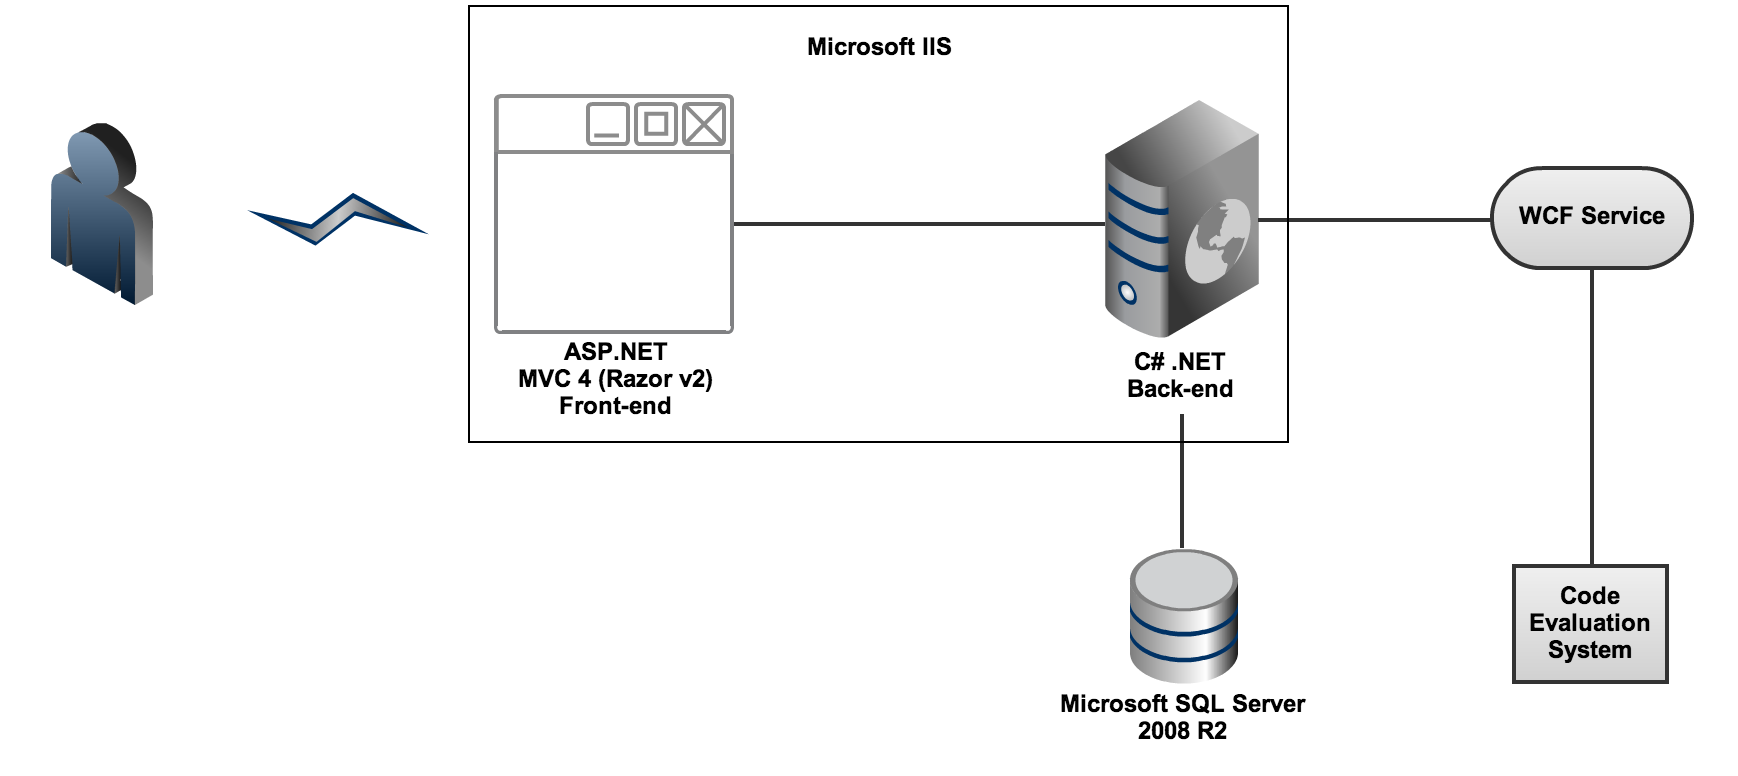
\includegraphics[width=0.9\linewidth]{chapters/media/overview.png}
	\caption{Overview of CELINE.}
	\label{fig:SystemOverview}
\end{figure}

Figure \ref{fig:SystemOverview} describes an overview of the system. The system uses a web based GUI for listing problems and submitting solutions to them. Going through this figure from left to right we can see that a user connects to the website through a web based GUI, which is built using a combination of ASP.NET MVC4 (Razor v2) technology and JavaScript. The system uses Microsoft IIS to enable this web support, which the standard web server software used in .NET. When the user submits code to solve a problem, that submission is saved to a database which is a Microsoft SQL Server 2008 R2 database. The submission is then forwarded to a WCF Service which in turn creates a new instance of the automatic grading system (built using C\#) using the submission as input. The automatic grader compiles the source if needed and runs the code. It then returns a status code generated from the submission, this is described in section \ref{subsec:status_codes}.


\subsection{The Web GUI and workflow}
The GUI is built using the ASP.NET MVC4 template. This saved both time and effort while still giving the website an easy to understand simplistic style.

\begin{figure}[h]
	\centering
	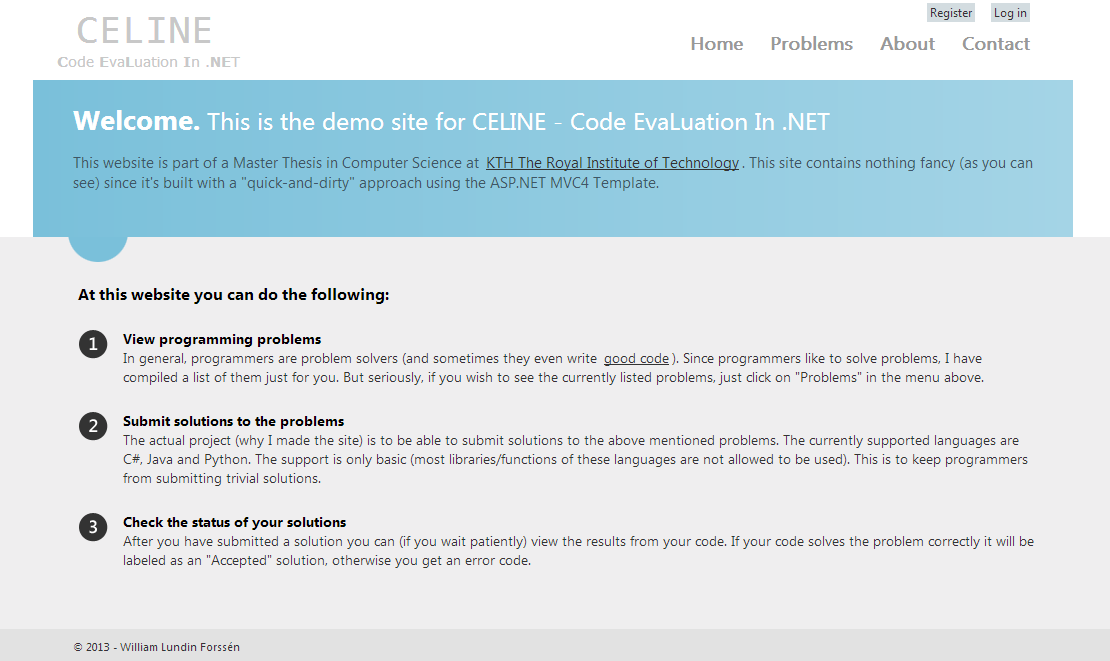
\includegraphics[width=1.0\textwidth]{chapters/media/celine_startpage.png}
	\caption{The start page of CELINE.}
	\label{fig:celine_startpage}
\end{figure}

In Figure \ref{fig:celine_startpage}, we see the start page. This is the page where applicants start their workflow. The middle area contains some informative text; the top right contains the site menu, the register and login buttons.

From the start page an applicant may click on the ``Problems'' text in the top-right corner which sends them to a page containing a list of problems, see Figure \ref{fig:celine_list_problems}.

\begin{figure}[h]
	\centering
	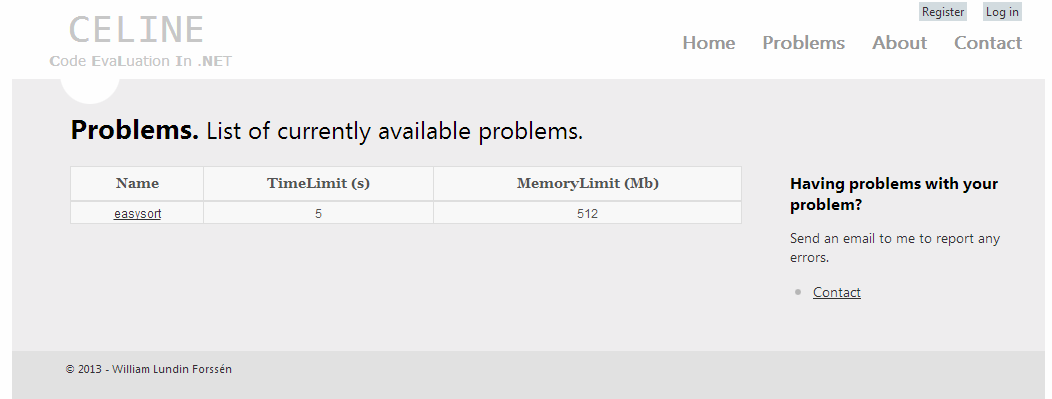
\includegraphics[width=1.0\textwidth]{chapters/media/celine_listproblemsCut.png}
	\caption{Listing of available problems page. This page is shown when a user clicks on the ``Problems'' text in the top-right. One of the available problems is called ``easysort''. }
	\label{fig:celine_list_problems}
\end{figure}

Should the applicant find a problem they want to solve, they simply click on that problem in the list to arrive at an information page containing that specific problem, see Figure \ref{fig:celine_easysort}. If the applicant wants to solve this particular problem they may click on the ``Submit solution'' button (visible on the right side).

\begin{figure}[h]
	\centering
	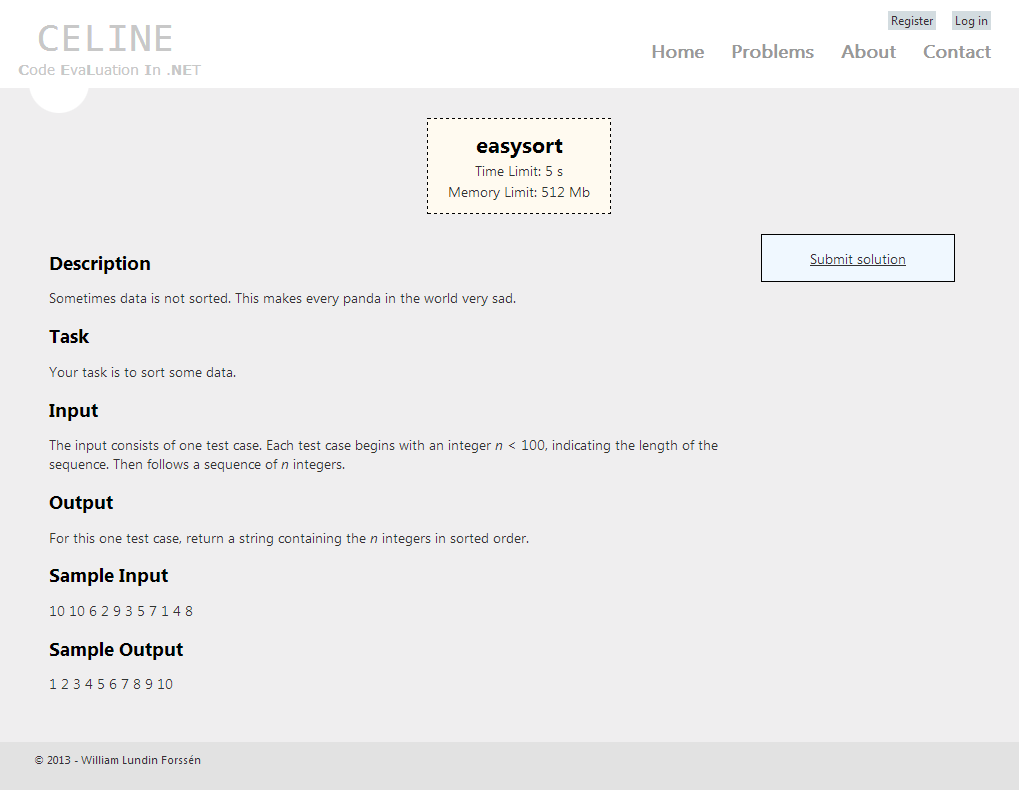
\includegraphics[width=1.0\textwidth]{chapters/media/celine_easysort.png}
	\caption{Problem information page. This is where applicants can read about the problem statement and get information regarding what to expect as input and what the system expects their solution to output.}
	\label{fig:celine_easysort}
\end{figure}

In Figure \ref{fig:celine_submit}, we see the submission form on the left side, this page contains some useful information on the right side concerning language-specific signatures. These signatures specify the point of entry for the application (where the execution of the code starts). Users are free to name this method to anything they see fit, the only limitation is that it takes a string as input and returns a string as output. This is discussed in further detail in section \ref{subsec:status_codes}.

\begin{figure}[h]
	\centering
	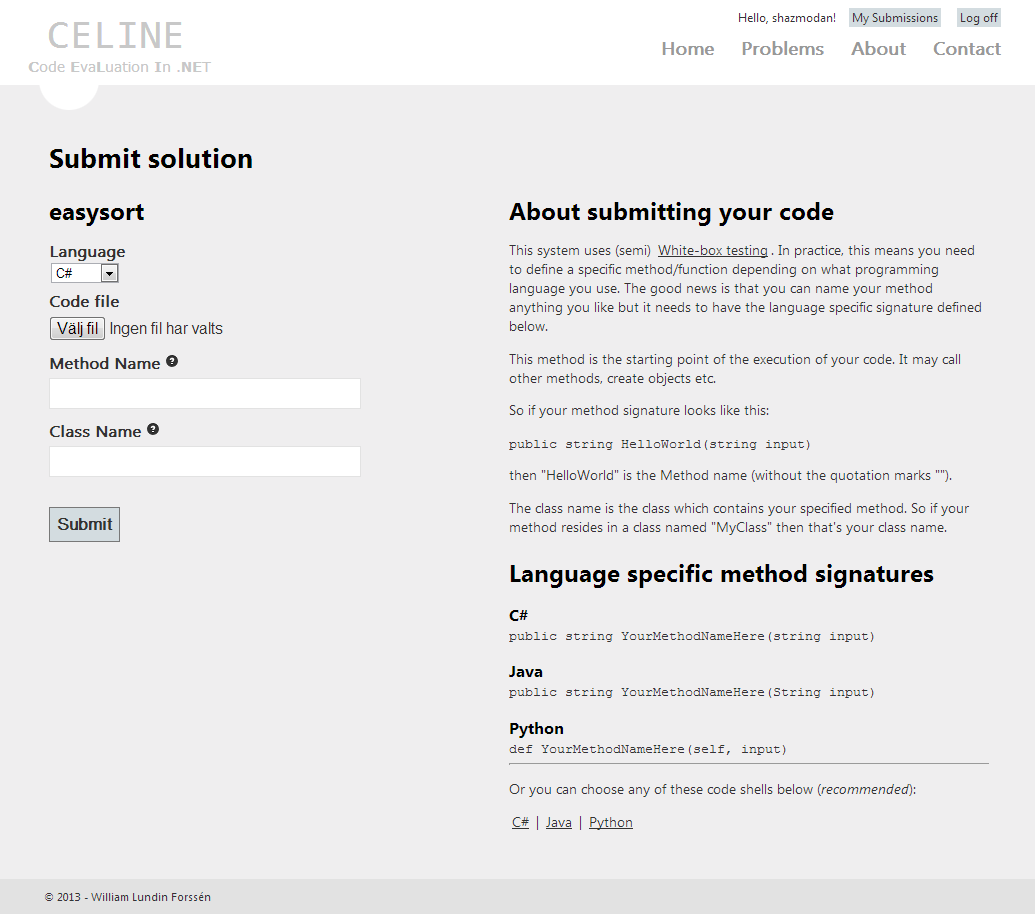
\includegraphics[width=1.0\textwidth]{chapters/media/celine_submit.png}
	\caption{Code submission page. This page provides the user with details regarding submitting a solution to a problem. The system requires that a specific programming language to be selected from the drop down list at the top, a main class name and a specified method signature (acting as the application's entry point).}
	\label{fig:celine_submit}
\end{figure}

When the applicant has submitted their solution, they are sent to a page where they can see all of their submissions, see Figure \ref{fig:celine_submissions}.

\begin{figure}[h]
	\centering
	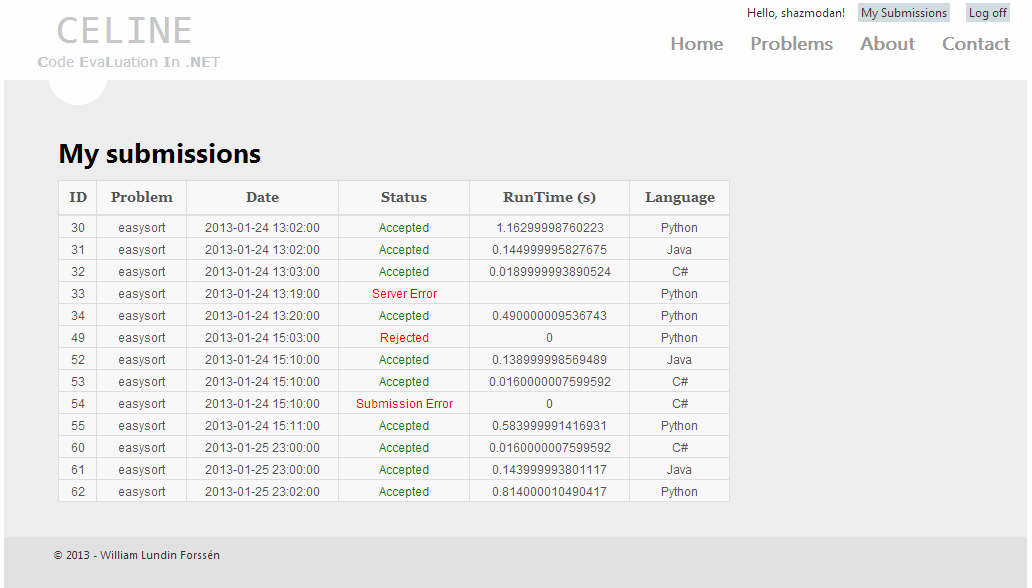
\includegraphics[width=1.0\textwidth]{chapters/media/celine_submissionsCut.png}
	\caption{All submissions page. This page displays a list of all submissions that an applicant has made. Each item in the list contains a unique id, the name of the problem, the date of when the submission was sent, the status code which indicates if the output was accepted or not, the time it took for the output to be produced and the language that was used.}
	\label{fig:celine_submit}
\end{figure}


\subsection{The Automatic Grading System}
When a user has submitted his or her code, it eventually reaches the AGS. Figure \ref{fig:flowchart} describes the flow of the most common paths for a submission through the system.

\begin{figure}[h]
	\centering
	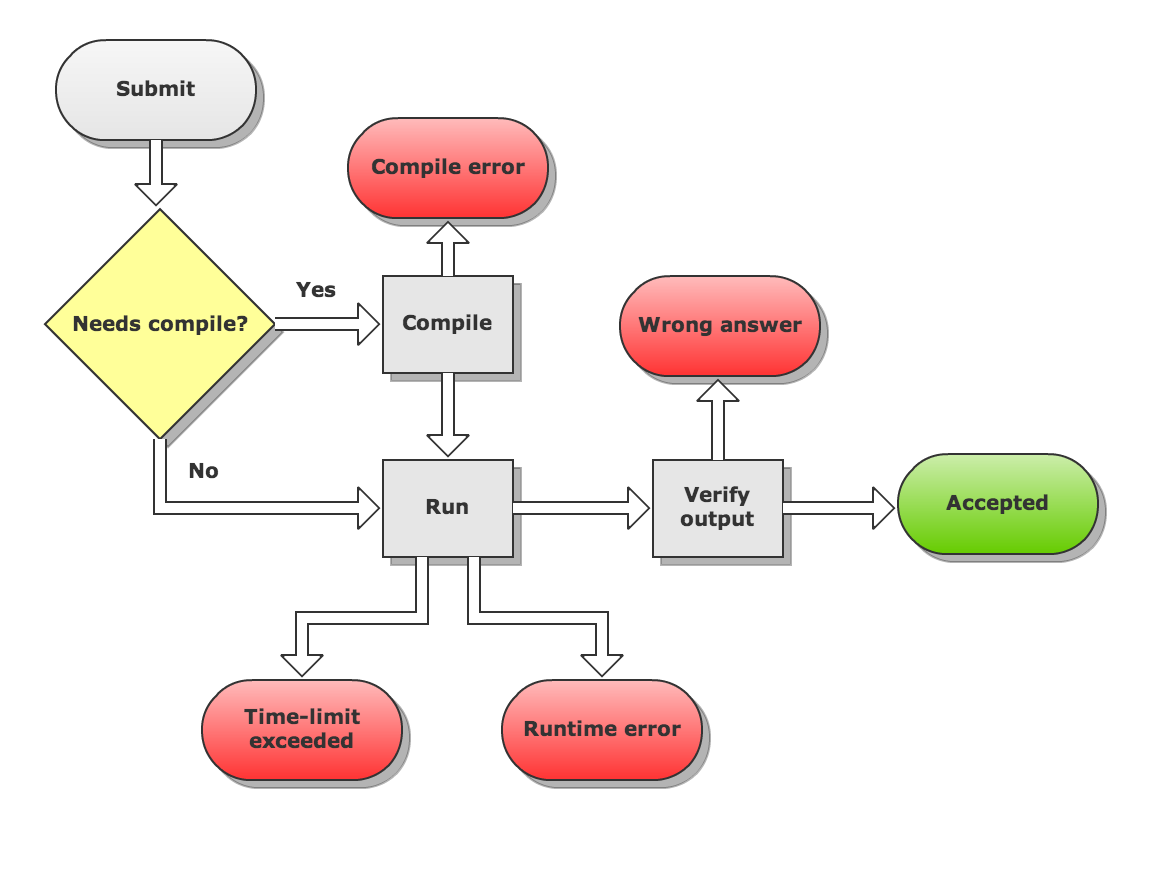
\includegraphics[width=0.8\linewidth]{chapters/media/flowchart.png}
	\caption{Common paths of problem flow in the AGS.}
	\label{fig:flowchart}
\end{figure}

Depending on the programming language, a compiler is chosen. The code is then compiled into an assembly file and loaded into a separate and secure Application Domain (AppDomain, see section \ref{subsec:security}). The AGS then invokes the user specified method with a string containing the test data. The AGS waits for the code to complete or for the problem to timeout. The timeout is problem specific and decided when the problem is created. It then compares the string returned by this method with another string containing what should be the correct output. If the strings match, the submission is regarded as being a success; otherwise it is regarded as a failure. The AGS then returns the appropriate status code.


\subsection{System-User Feedback} \label{subsec:status_codes}
The system gives feedback to the user in the form of a status code, one for each submission. The status code is a simplistic message that indicates whether the submission was successful or not. This system attempts to be more verbose on errors than other modern systems (described in section \ref{sec:todays_systems}). It uses grey-box testing, which is more prone to submission related errors, than black-box testing (commonly used in today's AGS:s). The concepts of white- and black-box testing are described more thoroughly in section \ref{subsec:whitebox_blackbox}. The following list contains the possible status codes:

\begin{itemize}
	\item Accepted - The code has compiled, run and gave the correct answer.
	\item Wrong Answer - The code has compiled and run but gave the wrong answer.
	\item Server Assembly Error - The AGS failed to build an assembly from the code file, thus making the code unable to run.
	\item Submission Error - The code tries to reference a code library that is not available/allowed.
	\item Illegal Operation - Occurs if the AGS detects a forbidden system call (e.g. accessing files, using the network etc...).
	\item Class or Function Error - Occurs if the class or method name does not correspond to the name provided by the user, thus resulting in the AGS being unable to invoke it.
	\item Time Limit Exceeded - The code ran longer than the time-limit for this problem allowed. This could be an indication that the code needs to be improved (performance wise). The time limit is decided by an administrator when the problem was created.
	\item Rejected - This is a general error which indicates that the AGS has been unable to determine why the submission failed.
	\item Server Error - This indicates that the AGS instance has crashed.
\end{itemize}

The status messages ``Server Assembly Error'', ``Submission Error'', ``Illegal operation'' and ``Class or Function Error'' are all related to incorrect formatting of the code by the user. These might be less verbose than one would like (e.g. each submission could have returned exactly where in the code the error occurred). Any more verbose feedback would have required an expansion of the scope of this thesis.

